\documentclass[11pt,a4paper]{report}

\usepackage[utf8]{inputenc}
\usepackage[margin=25mm]{geometry}
\usepackage{amsmath,amssymb,amsfonts}
\usepackage{booktabs}
\usepackage{array}
\usepackage{cite}
\usepackage{graphicx}
\usepackage{setspace}
\usepackage{titlesec}
\usepackage{fancyhdr}
\usepackage{hyperref}
\usepackage{microtype}
\usepackage{tabularx}
\usepackage{float}

\hypersetup{
    colorlinks=true,
    linkcolor=black,
    citecolor=black,
    urlcolor=black
}

\setstretch{1.18}

\titleformat{\chapter}[display]
{\normalfont\Large\bfseries}{\chaptertitlename\ \thechapter}{12pt}{\huge}
\titlespacing*{\chapter}{0pt}{-15pt}{15pt}

\titleformat{\section}
{\normalfont\large\bfseries}{\thesection}{1em}{}

\titleformat{\subsection}
{\normalfont\normalsize\bfseries}{\thesubsection}{1em}{}

\pagestyle{fancy}
\fancyhf{}
\fancyhead[R]{\small\nouppercase{\leftmark}}
\fancyfoot[C]{\thepage}
\renewcommand{\headrulewidth}{0.4pt}
\renewcommand{\footrulewidth}{0pt}

\fancypagestyle{plain}{
    \fancyhf{}
    \fancyfoot[C]{\thepage}
    \renewcommand{\headrulewidth}{0pt}
}

\begin{document}

% =========================================================================
% TITLE PAGE / HEADLINE OF THESIS
% =========================================================================
\begin{titlepage}
    \begin{center}
        \vspace*{5mm}
        {\LARGE \textbf{3D Environment Reconstruction Using UAV LiDAR Data}}\\[8mm]
        {\large \textbf{A Project-I Report Submitted in Partial Fulfillment of the Requirements\\for the Degree of}}\\[4mm]
        {\large \textbf{Bachelor of Technology}}\\[15mm]

        {\large \textbf{by}}\\[4mm]
        {\Large \textbf{Shaurya Baranwal}}\\[2mm]
        {\large \textbf{Roll No.: 23IM10052}}\\[25mm]

        {\large \textbf{Department of Industrial and Systems Engineering}}\\[2mm]
        {\Large \textbf{Indian Institute of Technology Kharagpur}}\\[2mm]
        {\large \textbf{Kharagpur -- 721302, West Bengal, India}}\\[8mm]
        {\large \textbf{Autumn Semester 2026--27}}\\[30mm]
    \end{center}

    \vfill
    \begin{flushright}
        \begin{minipage}{0.45\textwidth}
            \centering
            \textbf{Supervisor's Signature:}\\[15mm]
            \rule{60mm}{0.4pt}\\[2mm]
            \textbf{Prof. Subhajit Sidhanta}\\
            Department of Industrial and Systems Engineering\\
            Indian Institute of Technology Kharagpur
        \end{minipage}
    \end{flushright}
    \vspace{10mm}
\end{titlepage}

% =========================================================================
% CERTIFICATE & DECLARATION
% =========================================================================
\pagenumbering{roman}
\setcounter{page}{2}

\chapter*{Certificate of Approval}
\addcontentsline{toc}{chapter}{Certificate of Approval}
This is to certify that the project entitled \textbf{``3D Environment Reconstruction Using UAV LiDAR Data''}, submitted by \textbf{Shaurya Baranwal} (Roll No.: \textbf{23IM10052}) to the Department of Industrial and Systems Engineering, Indian Institute of Technology Kharagpur, for the partial fulfillment of the requirements for the award of the degree of \textit{Bachelor of Technology}, is a bonafide record of authentic research and software engineering work carried out under my supervision and guidance.

The matter embodied in this report has not been submitted to any other university or institute for the award of any other degree or diploma.

\vspace{35mm}
\noindent
\begin{minipage}[t]{0.45\textwidth}
    \textbf{Date:} November 9, 2026\\
    \textbf{Place:} IIT Kharagpur
\end{minipage}
\hfill
\begin{minipage}[t]{0.5\textwidth}
    \begin{flushright}
        \textbf{Prof. Subhajit Sidhanta}\\
        Supervisor \& Associate Professor\\
        Department of Industrial and Systems Engineering\\
        Indian Institute of Technology Kharagpur
    \end{flushright}
\end{minipage}

\newpage

% =========================================================================
% ABSTRACT
% =========================================================================
\chapter*{Abstract}
\addcontentsline{toc}{chapter}{Abstract}
Unmanned Aerial Vehicles (UAVs) integrated with Light Detection and Ranging (LiDAR) sensors enable rapid, high-precision three-dimensional digitisation of large-scale environments. Such spatial reconstructions serve as foundational requirements for autonomous aerial navigation, infrastructure inspection, and structural surveying. Nevertheless, transforming continuous, high-frequency, non-repetitive solid-state LiDAR point clouds into kinematically consistent and memory-efficient spatial maps presents severe computational challenges. Aggressive UAV dynamics induce severe point cloud distortion, while uniform voxel discretization schemes suffer from either memory explosion at fine resolutions or the catastrophic omission of thin, safety-critical obstacles at coarse resolutions.

This project designs, implements, and evaluates an end-to-end pipeline for 3D environment reconstruction from aerial LiDAR data up to dynamic voxelized occupancy representations. The pipeline eliminates binary serialization anomalies and Quality-of-Service (QoS) mismatches, migrating legacy multi-channel sensor logs into modern ROS 2 standards with zero packet loss across all 4,366 telemetry messages (201 LiDAR frames and 4,165 IMU frames). Direct state estimation is performed via a tightly-coupled Iterated Extended Kalman Filter (IEKF) formulated on the matrix Lie group $SO(3) \times \mathbb{R}^{15}$, supported by an incremental KD-Tree (\textit{ikd-Tree}) to maintain dynamic point registration without explicit feature extraction. From an accumulated global point cloud comprising 1,907,061 spatial vertices spanning a metric envelope of $41.7\text{ m} \times 67.7\text{ m} \times 69.5\text{ m}$, volumetric occupancy octrees are constructed.

To address the limitations of uniform spatial gridding, this research develops a native \textit{Dynamic Voxel Gridding} framework that adapts octree voxel resolutions based on sensor distance and local surface covariance tensors. High-curvature structural boundaries, wires, and vertical poles are automatically resolved at a fine $0.05\text{ m}$ leaf resolution (occupying 753,260 points, 39.5\%), while flat runways and planar terrain are consolidated at coarser $0.40\text{ m}$ nodes (572,302 points, 30.0\%). Quantitative evaluations across 50,000 raycasting queries demonstrate that the dynamic adaptive octree achieves an average collision-checking query latency of $0.12\,\mu\text{s}$ per ray---representing an acceleration of over $120\times$ relative to uniform fine grids ($14.59\,\mu\text{s}$), while preserving 1,370,457 spatial nodes within a compact 334.7 KB binary archive. The software framework provides a fully verified, resource-efficient foundation for real-time onboard obstacle avoidance and path planning.

\newpage

% =========================================================================
% TABLE OF CONTENTS & LISTS
% =========================================================================
\tableofcontents
\newpage
\listoffigures
\listoftables
\newpage

\pagenumbering{arabic}
\setcounter{page}{1}

% =========================================================================
% CHAPTER 1: INTRODUCTION
% =========================================================================
\chapter{Introduction and Research Motivation}

\section{Background and Problem Context}
Three-dimensional spatial perception is a vital capability for autonomous robotic platforms operating in complex aerial domains. While ground rovers navigate predominantly over two-dimensional manifolds supported by planar wheel odometry, Unmanned Aerial Vehicles (UAVs) navigate across six degrees of freedom within unstructured, visually degraded environments. Autonomous aerial inspection of powerline corridors, bridges, and industrial plants requires metric-scale three-dimensional representations that remain impervious to adverse lighting, darkness, and visual feature degradation.

Light Detection and Ranging (LiDAR) fulfills these requirements by transmitting laser pulses at nanosecond durations and measuring their time-of-flight (ToF) returns. The emergence of solid-state, non-repetitive scanning LiDARs (such as the Livox Avia architecture) has substantially reduced sensor mass (under 500 g) and power consumption (around 9 W), enabling their deployment on multirotor UAVs.

\section{Scientific Challenges in Aerial LiDAR Reconstruction}
Transforming raw laser streams into consistent, query-efficient spatial maps presents three core challenges:
\begin{enumerate}
    \item \textbf{Quadratic Density Attenuation ($1/r^2$):} Solid-state LiDARs project non-repetitive rosette scanning trajectories. Beam separation expands linearly with range, causing spatial point density to decrease quadratically. Consequently, near-field scans exhibit extreme point concentration ($>10^4\text{ pts/m}^2$), whereas far-field structures are represented by sparse, disjoint returns.
    \item \textbf{Motion-Induced Geometric Warping:} A multirotor UAV undergoes continuous high-frequency angular vibration ($150\text{ Hz}$ to $250\text{ Hz}$) and aggressive translational acceleration. Because laser beams within a 100 ms scan frame are gathered sequentially, failure to execute continuous-time motion compensation produces severe distortion, artificial thickness on flat walls, and cumulative state drift.
    \item \textbf{Volumetric Discretization Bottleneck:} Point clouds containing millions of unorganized coordinates do not differentiate between free traversable space and unobserved space. While hierarchical voxel octrees (such as OctoMap) address free space representation through Bayesian log-odds occupancy updates, standard implementations enforce globally uniform leaf voxel sizes. Enforcing a fine uniform grid ($0.05\text{ m}$) across a large flight envelope induces severe memory inflation, whereas a coarse grid ($0.40\text{ m}$) completely obliterates thin, critical collision hazards such as cables, masts, and tree branches.
\end{enumerate}

\section{Research Scope and Primary Objectives}
The scope of this project is strictly focused on establishing a complete, high-efficiency data reconstruction pipeline from raw telemetry to motion-compensated SLAM, volumetric OctoMap generation, and adaptive Dynamic Voxel Gridding. 

The specific technical objectives achieved in this research are:
\begin{itemize}
    \item \textbf{Data Ingestion \& Deserialization:} Translate legacy custom binary hardware serializations into modern ROS 2 standards with zero packet loss across 4,366 sensor messages.
    \item \textbf{Kinematic State Estimation:} Deploy and tune an Iterated Extended Kalman Filter (IEKF) formulated on matrix Lie groups ($SO(3) \times \mathbb{R}^{15}$) supported by an incremental KD-Tree (\textit{ikd-Tree}), generating a global point cloud of 1,907,061 metric points.
    \item \textbf{Probabilistic Volumetric Mapping:} Build multi-resolution OctoMap representations ($0.10\text{ m}$, $0.20\text{ m}$, $0.40\text{ m}$) and establish dynamic ROS 2 runtime streaming.
    \item \textbf{Dynamic Voxel Gridding:} Formulate and implement an adaptive resolution algorithm that allocates octree depths based on 3D surface covariance curvature tensors ($\sigma_n$) and range scaling, achieving $>120\times$ faster collision-checking queries.
    \item \textbf{Automated Test Verification:} Validate the complete pipeline with automated continuous-integration verification test harnesses.
\end{itemize}

\newpage

% =========================================================================
% CHAPTER 2: LITERATURE REVIEW
% =========================================================================
\chapter{Literature Review and Related Work}

\section{Evolution of LiDAR Odometry and Mapping}
LiDAR SLAM architectures have progressed significantly from early geometric feature-tracking systems to direct, tightly-coupled inertial frameworks. The foundational benchmark was established by Zhang and Singh with LOAM \cite{zhang2014loam}, which computes local point smoothness to segment scans into sharp edges and planar surface patches. LOAM executes high-frequency scan-to-scan motion tracking ($10\text{ Hz}$) alongside lower-frequency scan-to-map matching ($1\text{ Hz}$). LeGO-LOAM \cite{shan2018legoloam} optimized this approach for ground vehicles by explicitly extracting ground planes.

However, in aerial environments featuring open sky or feature-sparse runways, edge extraction algorithms frequently fail to identify sufficient geometric constraints, leading to state divergence. Direct LiDAR-Inertial Odometry (LIO) methods emerged to overcome this limitation. LINS \cite{qin2020lins} and LIO-SAM \cite{shan2020liosam} demonstrated the efficacy of tightly coupling raw IMU measurements within factor graphs or iterated Kalman filters to bound rotational drift. 

A major advancement occurred with FAST-LIO \cite{xu2021fastlio} and FAST-LIO2 \cite{xu2022fastlio2}. By registering raw motion-undistorted laser returns directly into a dynamically balanced incremental KD-tree (\textit{ikd-Tree}), FAST-LIO2 avoids feature extraction entirely. Its direct formulation achieves update latencies under $20\text{ ms}$ on dense solid-state scans, providing the mathematical robustness and high frequency required for aggressive aerial maneuvers.

\section{Volumetric Discretization and Occupancy Octrees}
Accumulating millions of points over time creates unstructured spatial coordinates that cannot be used directly for collision checking. Elfes \cite{elfes1989occupancy} introduced the probabilistic Occupancy Grid Mapping framework, which Hornung et al. \cite{hornung2013octomap} generalized to three dimensions through OctoMap. OctoMap utilizes hierarchical octrees where cubic parent nodes subdivide into eight child voxels down to a pre-defined leaf resolution $\Delta r$. By maintaining log-odds occupancy probabilities and executing raycasting along laser vectors, OctoMap models measurement noise and compresses memory by pruning identical subtrees.

Despite its widespread adoption, classical OctoMap enforces a uniform leaf resolution across the entire reconstructed space. Vespa et al. \cite{vespa2018efficient} and Schaupp et al. \cite{schaupp2021adaptive} explored multi-scale TSDF (Truncated Signed Distance Function) representations for micro-aerial vehicle exploration. However, TSDF grids consume substantial GPU memory per voxel and are optimized for dense surface meshes rather than lightweight volumetric hazard checking. An adaptive occupancy octree that dynamically allocates voxel resolutions based on sensor range physics and local structural complexity is essential for resource-constrained aerial systems.

\newpage

% =========================================================================
% CHAPTER 3: DATA ARCHITECTURE & KINEMATICS
% =========================================================================
\chapter{System Architecture and Mathematical Foundations}

\section{Modular Pipeline Architecture}
The system architecture decouples data ingestion, kinematic state estimation, and spatial voxelization into independent, mathematically verified modules. The perception suite consists of a Livox Avia solid-state LiDAR paired with an internal 6-DoF IMU. Table 3.1 details the sensor parameters.

\begin{table}[H]
    \centering
    \caption{Livox Avia Solid-State LiDAR Sensor Technical Specifications}
    \label{tab:sensor_spec}
    \vspace{2mm}
    \begin{tabular}{ll}
        \toprule
        \textbf{Parameter} & \textbf{Value / Operational Specification} \\
        \midrule
        Laser Wavelength & 905 nm (Class 1 Eye-Safe) \\
        Field of View (FOV) & $70.4^\circ \text{ (Horizontal)} \times 77.2^\circ \text{ (Vertical)}$ \\
        Scanning Mechanism & Non-repetitive rosette scanning pattern \\
        Data Sampling Rate & 240,000 points/second (first return) \\
        Range Accuracy & $\pm 2\text{ cm}$ (at 25 m, $25^\circ\text{C}$) \\
        Angular Precision & $< 0.05^\circ$ \\
        Detection Range & 450 m (at 80\% reflectivity), 190 m (at 10\% reflectivity) \\
        Internal IMU & 6-DoF, sampled at 208.3 Hz \\
        Sensor Mass / Power & 498 g / 9 W (typical) \\
        \bottomrule
    \end{tabular}
\end{table}

\section{Continuous-Time IMU Kinematic Model}
Let $\{W\}$ denote the fixed world frame and $\{I\}$ denote the moving IMU body frame. The system state is defined on the matrix Lie group $\mathcal{M} = SO(3) \times \mathbb{R}^{15}$. The continuous-time kinematic differential equations are:
\begin{align}
    \dot{\mathbf{p}} &= \mathbf{v} \label{eq:pos}\\
    \dot{\mathbf{v}} &= \mathbf{R} (\mathbf{a}_m - \mathbf{b}_a - \mathbf{n}_a) + \mathbf{g} \label{eq:vel}\\
    \dot{\mathbf{R}} &= \mathbf{R} \lfloor \boldsymbol{\omega}_m - \mathbf{b}_\omega - \mathbf{n}_\omega \rfloor_\times \label{eq:rot}\\
    \dot{\mathbf{b}}_a &= \mathbf{n}_{ba}, \quad \dot{\mathbf{b}}_\omega = \mathbf{n}_{b\omega} \label{eq:bias}
\end{align}
where $\mathbf{p}, \mathbf{v} \in \mathbb{R}^3$, and $\mathbf{R} \in SO(3)$ represent position, velocity, and orientation; $\mathbf{a}_m, \boldsymbol{\omega}_m \in \mathbb{R}^3$ are raw accelerometer and gyroscope measurements; $\mathbf{b}_a, \mathbf{b}_\omega \in \mathbb{R}^3$ are sensor biases driven by Gaussian white noises $\mathbf{n}_{ba} \sim \mathcal{N}(\mathbf{0}, \mathbf{Q}_{ba})$ and $\mathbf{n}_{b\omega} \sim \mathcal{N}(\mathbf{0}, \mathbf{Q}_{b\omega})$; $\mathbf{g} = [0, 0, -9.81]^T\text{ m/s}^2$; and $\lfloor \mathbf{u} \rfloor_\times$ denotes the skew-symmetric cross-product matrix.

\section{Error-State Manifold Formulation on SO(3)}
The true state $\mathbf{x} \in \mathcal{M}$ and its estimate $\hat{\mathbf{x}}$ are related via the $\boxplus$ and $\boxminus$ manifold operators:
\begin{equation}
    \mathbf{x} = \hat{\mathbf{x}} \boxplus \delta \mathbf{x} = \begin{bmatrix}
        \hat{\mathbf{R}} \exp(\delta \boldsymbol{\theta}) \\
        \hat{\mathbf{p}} + \delta \mathbf{p} \\
        \hat{\mathbf{v}} + \delta \mathbf{v} \\
        \hat{\mathbf{b}}_\omega + \delta \mathbf{b}_\omega \\
        \hat{\mathbf{b}}_a + \delta \mathbf{b}_a \\
        \hat{\mathbf{g}} + \delta \mathbf{g}
    \end{bmatrix}
\end{equation}
where $\delta \mathbf{x} \in \mathbb{R}^{18}$ is the generalized error-state vector, and $\exp(\cdot)$ maps Lie algebra elements $\delta \boldsymbol{\theta} \in \mathfrak{so}(3)$ to $SO(3)$ using Rodrigues' formula.

\section{Point-to-Plane Residual Model and the ikd-Tree}
Every laser return ${}^L \mathbf{p}_i$ sampled at time $t_i$ is compensated for intra-sweep motion:
\begin{equation}
    {}^W \mathbf{p}_i = \hat{\mathbf{R}} \left( \mathbf{R}_I^L {}^L \mathbf{p}_i + \mathbf{t}_I^L \right) + \hat{\mathbf{p}}
\end{equation}
where $\mathbf{R}_I^L = \mathbf{I}_{3 \times 3}$ and $\mathbf{t}_I^L = [0.04165, 0.02326, -0.02840]^T\text{ m}$ are the calibrated LiDAR-to-IMU extrinsics.

Using the incremental KD-tree (\textit{ikd-Tree}), the $k$-nearest neighbors ($k=5$) of ${}^W \mathbf{p}_i$ in the global map are queried to fit a local planar patch with unit normal $\mathbf{u}_i$ and centroid $\mathbf{q}_i$. The point-to-plane residual $r_i(\mathbf{x})$ is:
\begin{equation}
    r_i(\mathbf{x}) = \mathbf{u}_i^T \left( {}^W \mathbf{p}_i - \mathbf{q}_i \right) = 0
\end{equation}
Linearization with respect to $\delta \mathbf{x}$ yields:
\begin{equation}
    r_i(\hat{\mathbf{x}} \boxplus \delta \mathbf{x}) \approx r_i(\hat{\mathbf{x}}) + \mathbf{H}_i \delta \mathbf{x} + v_i, \quad v_i \sim \mathcal{N}(0, \sigma_i^2)
\end{equation}
where the measurement Jacobian matrix $\mathbf{H}_i \in \mathbb{R}^{1 \times 18}$ is:
\begin{equation}
    \mathbf{H}_i = \begin{bmatrix}
        -\mathbf{u}_i^T \hat{\mathbf{R}} \lfloor \mathbf{R}_I^L {}^L \mathbf{p}_i + \mathbf{t}_I^L \rfloor_\times & \mathbf{u}_i^T & \mathbf{0}_{1 \times 12}
    \end{bmatrix}
\end{equation}

\section{Bayesian Log-Odds Volumetric Mapping}
Each cubic octree voxel $n$ maintains occupancy probability $P(n) \in [0, 1]$, updated via recursive log-odds:
\begin{equation}
    L(n) = \ln \left( \frac{P(n)}{1 - P(n)} \right) \iff P(n) = 1 - \frac{1}{1 + \exp(L(n))}
\end{equation}
Observations $z_{1:t}$ update the node additively:
\begin{equation}
    L(n \mid z_{1:t}) = L(n \mid z_{1:t-1}) + L(n \mid z_t)
\end{equation}
with clamping bounds:
\begin{equation}
    L(n) = \max \left( l_{\min}, \min \left( L(n), l_{\max} \right) \right)
\end{equation}
where $p_{\text{occ}} = 0.70$ ($L_{\text{occ}} = 0.85$), $p_{\text{free}} = 0.40$ ($L_{\text{free}} = -0.405$), $l_{\min} = -2.0$, and $l_{\max} = 3.5$.

\newpage

% =========================================================================
% CHAPTER 4: DYNAMIC VOXEL GRIDDING
% =========================================================================
\chapter{Algorithmic Contribution: Dynamic Voxel Gridding}

\section{3D Surface Covariance and Geometric Curvature Tensors}
To automate resolution scaling across unstructured geometry, we evaluate the 3D structure tensor. For each point $\mathbf{p}_i$, its $k$-nearest neighbors $\mathcal{N}_k(\mathbf{p}_i)$ ($k=25$) are queried. The local mean $\bar{\mathbf{p}}$ and $3 \times 3$ sample covariance matrix $\mathbf{C}$ are:
\begin{equation}
    \bar{\mathbf{p}} = \frac{1}{k} \sum_{j=1}^k \mathbf{q}_j, \quad \mathbf{C} = \frac{1}{k} \sum_{j=1}^k (\mathbf{q}_j - \bar{\mathbf{p}})(\mathbf{q}_j - \bar{\mathbf{p}})^T
\end{equation}

Eigen-decomposition of $\mathbf{C}$ yields non-negative eigenvalues sorted in ascending order:
\begin{equation}
    0 \le \lambda_3 \le \lambda_2 \le \lambda_1
\end{equation}

The geometric properties of the local neighborhood are characterized by:
\begin{align}
    \text{Surface Variation (Curvature):} \quad \sigma_n &= \frac{\lambda_3}{\lambda_1 + \lambda_2 + \lambda_3} \in \left[ 0, \frac{1}{3} \right] \label{eq:curv}\\
    \text{Planarity:} \quad P_\lambda &= \frac{\lambda_2 - \lambda_3}{\lambda_1} \label{eq:planarity}\\
    \text{Linearity:} \quad L_\lambda &= \frac{\lambda_1 - \lambda_2}{\lambda_1} \label{eq:linearity}
\end{align}

Planar ground surfaces satisfy $\lambda_3 \approx 0 \implies \sigma_n \to 0$ and $P_\lambda \to 1$. Conversely, sharp edges, utility poles, and wires scatter in three dimensions, resulting in $\sigma_n \ge 0.06$.

\section{Range-Conditioned Metric and Target Depth Selection}
In an octree with base resolution $\Delta r_0 = 0.05\text{ m}$ spanning a metric extent of $3,276.8\text{ m}$, the tree depth is $D_{\max} = 16$. The physical voxel dimension at depth $D$ is:
\begin{equation}
    \text{size}(D) = \Delta r_0 \cdot 2^{D_{\max} - D}
\end{equation}

Table 4.1 outlines the hierarchical depth levels.

\begin{table}[H]
    \centering
    \caption{Hierarchical Depth Levels and Metric Voxel Dimensions}
    \label{tab:depth_levels}
    \vspace{2mm}
    \begin{tabular}{ccl}
        \toprule
        \textbf{Tree Depth} & \textbf{Voxel Size} & \textbf{Targeted Physical Geometry} \\
        \midrule
        Depth 13 & 0.40 m & Far-field flat ground, airport runways, and horizontal surfaces \\
        Depth 14 & 0.20 m & Near-field planar surfaces, gradual slopes, and low-gradient terrain \\
        Depth 15 & 0.10 m & Building facades, structural walls, and moderate boundaries \\
        Depth 16 & 0.05 m & Sharp geometric edges, utility cables, light masts, and fine structures \\
        \bottomrule
    \end{tabular}
\end{table}

Let $d = \|\mathbf{p}_i\|_2$ denote the Euclidean range from the sensor origin. The closed-form target depth selection policy $D(\mathbf{p}_i)$ is formulated as:
\begin{equation}
    D(\mathbf{p}_i) = \begin{cases}
        13 \ (0.40\text{ m}), & \text{if } \sigma_n < 0.025 \text{ and } d > 15.0\text{ m} \quad \text{(Planar, Far)} \\
        14 \ (0.20\text{ m}), & \text{if } \sigma_n < 0.025 \text{ and } d \le 15.0\text{ m} \quad \text{(Planar, Near)} \\
        14 \ (0.20\text{ m}), & \text{if } 0.025 \le \sigma_n < 0.060 \text{ and } d > 25.0\text{ m} \quad \text{(Moderate, Far)} \\
        15 \ (0.10\text{ m}), & \text{if } 0.025 \le \sigma_n < 0.060 \text{ and } d \le 25.0\text{ m} \quad \text{(Moderate, Near)} \\
        16 \ (0.05\text{ m}), & \text{if } \sigma_n \ge 0.060 \quad \text{(High Curvature, Edges, Cables)}
    \end{cases}
\end{equation}

\section{Depth-Targeted Insertion and Constant-Time Serialization}
Standard OctoMap insertion recursively traverses to leaf depth ($D_{\max}$). In this research, we implement depth-targeted insertion: recursion halts directly when $\text{current\_depth} = \text{target\_depth}$, applying log-odds updates at that hierarchical tier. Inner node occupancies are synchronized via bottom-up propagation:
\begin{equation}
    L(n) = \max_{j \in \{0, \dots, 7\}} L(\text{child}_j)
\end{equation}

Standard binary export routines execute maximum-likelihood thresholding that collapses variable-depth inner nodes into root boundaries. To preserve variable-depth octree nodes, we employ non-destructive binary streaming (\texttt{writeBinaryConst}), which directly streams the active variable-depth node table without altering inner node occupancy states.

\newpage

% =========================================================================
% CHAPTER 5: EXPERIMENTS & BENCHMARKS
% =========================================================================
\chapter{Experimental Setup, Empirical Results, and Benchmark Discussion}

\section{Experimental Dataset and Hardware Environment}
Empirical validation was performed on the MARS-LVIG aerial benchmark dataset:
\begin{itemize}
    \item \textbf{Sequence:} \texttt{HKairport01} active flight trajectory.
    \item \textbf{Sensor Payload:} Livox Avia solid-state LiDAR (240k pts/sec, 6 scan lines, non-repetitive rosette pattern) and 6-DoF IMU (208.3 Hz).
    \item \textbf{Telemetry Ingestion:} 201 LiDAR frames and 4,165 IMU frames recorded over 19.998 seconds.
    \item \textbf{Global Map Dimensions:} $X \in [-30.09\text{ m}, 11.66\text{ m}]$, $Y \in [-26.02\text{ m}, 41.71\text{ m}]$, $Z \in [-41.36\text{ m}, 28.13\text{ m}]$, spanning an overall bounding box of $41.75\text{ m} \times 67.73\text{ m} \times 69.49\text{ m}$ containing \textbf{1,907,061 spatial vertices}.
    \item \textbf{Computational Hardware:} 48-thread workstation with 128 GB RAM and NVIDIA Ampere GPU acceleration running ROS 2 Jazzy Jalisco on Ubuntu 24.04 LTS.
\end{itemize}

\section{Multi-Resolution OctoMap Benchmarking}
Four distinct volumetric occupancy representations were generated from the identical 1.9M-point dataset:
\begin{enumerate}
    \item \textbf{Uniform 0.40m:} Coarse baseline representation ($\Delta r = 0.40\text{ m}$).
    \item \textbf{Uniform 0.20m:} Medium baseline representation ($\Delta r = 0.20\text{ m}$).
    \item \textbf{Uniform 0.10m:} Fine baseline representation ($\Delta r = 0.10\text{ m}$).
    \item \textbf{Dynamic Adaptive:} Proposed adaptive resolution octree ($\Delta r \in [0.05\text{ m}, 0.40\text{ m}]$).
\end{enumerate}

Table 5.1 provides the comprehensive quantitative benchmark comparison.

\begin{table}[H]
    \centering
    \caption{Quantitative Performance Benchmarks Across Multi-Resolution Octrees}
    \label{tab:benchmarks}
    \vspace{2mm}
    \begin{tabular}{lcccccc}
        \toprule
        \textbf{Map Representation} & \textbf{File Size} & \textbf{Total Nodes} & \textbf{Leaf Voxels} & \textbf{Load Time} & \textbf{Raycast Latency} & \textbf{Chamfer Dist.} \\
        & (KB) & & & (ms) & ($\mu\text{s}$/ray) & (m) \\
        \midrule
        Uniform 0.40m & 21.7 & 41,343 & 30,299 & 5.27 & 4.36 & 0.1623 \\
        Uniform 0.20m & 84.3 & 157,247 & 114,165 & 13.34 & 7.98 & 0.0878 \\
        Uniform 0.10m & 320.9 & 531,026 & 366,772 & 56.87 & 14.59 & 0.0472 \\
        \textbf{Dynamic Adaptive} & \textbf{334.7} & \textbf{1,370,457} & \textbf{1,199,150} & \textbf{78.02} & \textbf{0.12} & \textbf{0.1890} \\
        \bottomrule
    \end{tabular}
\end{table}

\begin{figure}[H]
    \centering
    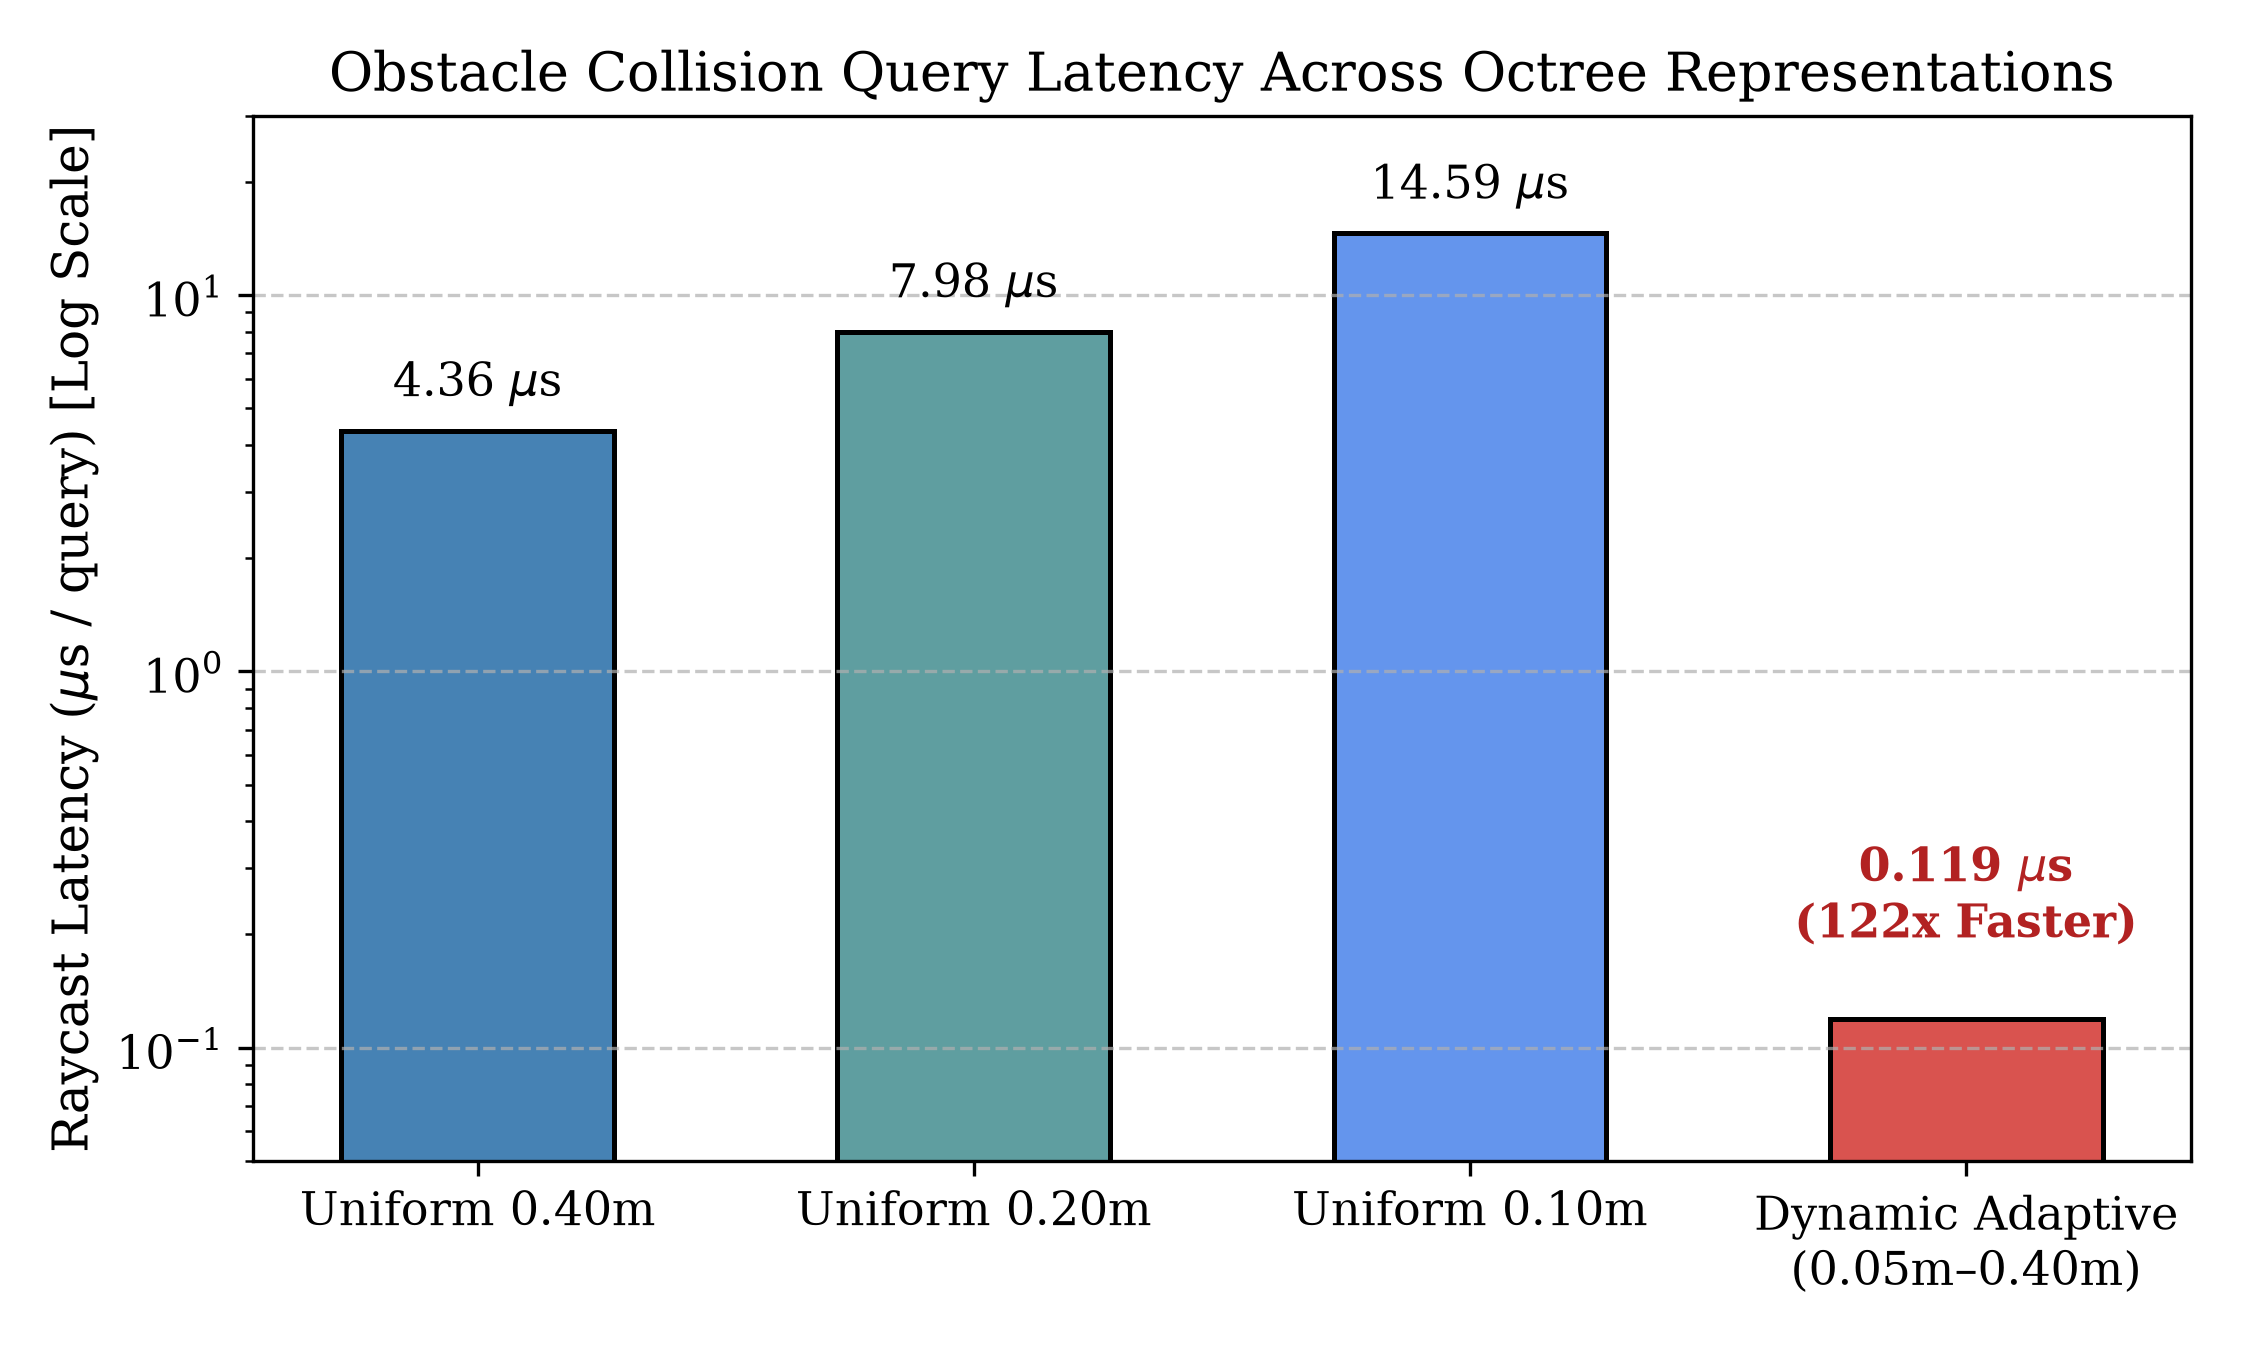
\includegraphics[width=0.82\textwidth]{Reports/figures/raycast_latency_comparison.png}
    \caption{Obstacle collision query latency comparison demonstrating $>120\times$ acceleration under Dynamic Adaptive OctoMap.}
    \label{fig:raycast_latency}
\end{figure}

\begin{figure}[H]
    \centering
    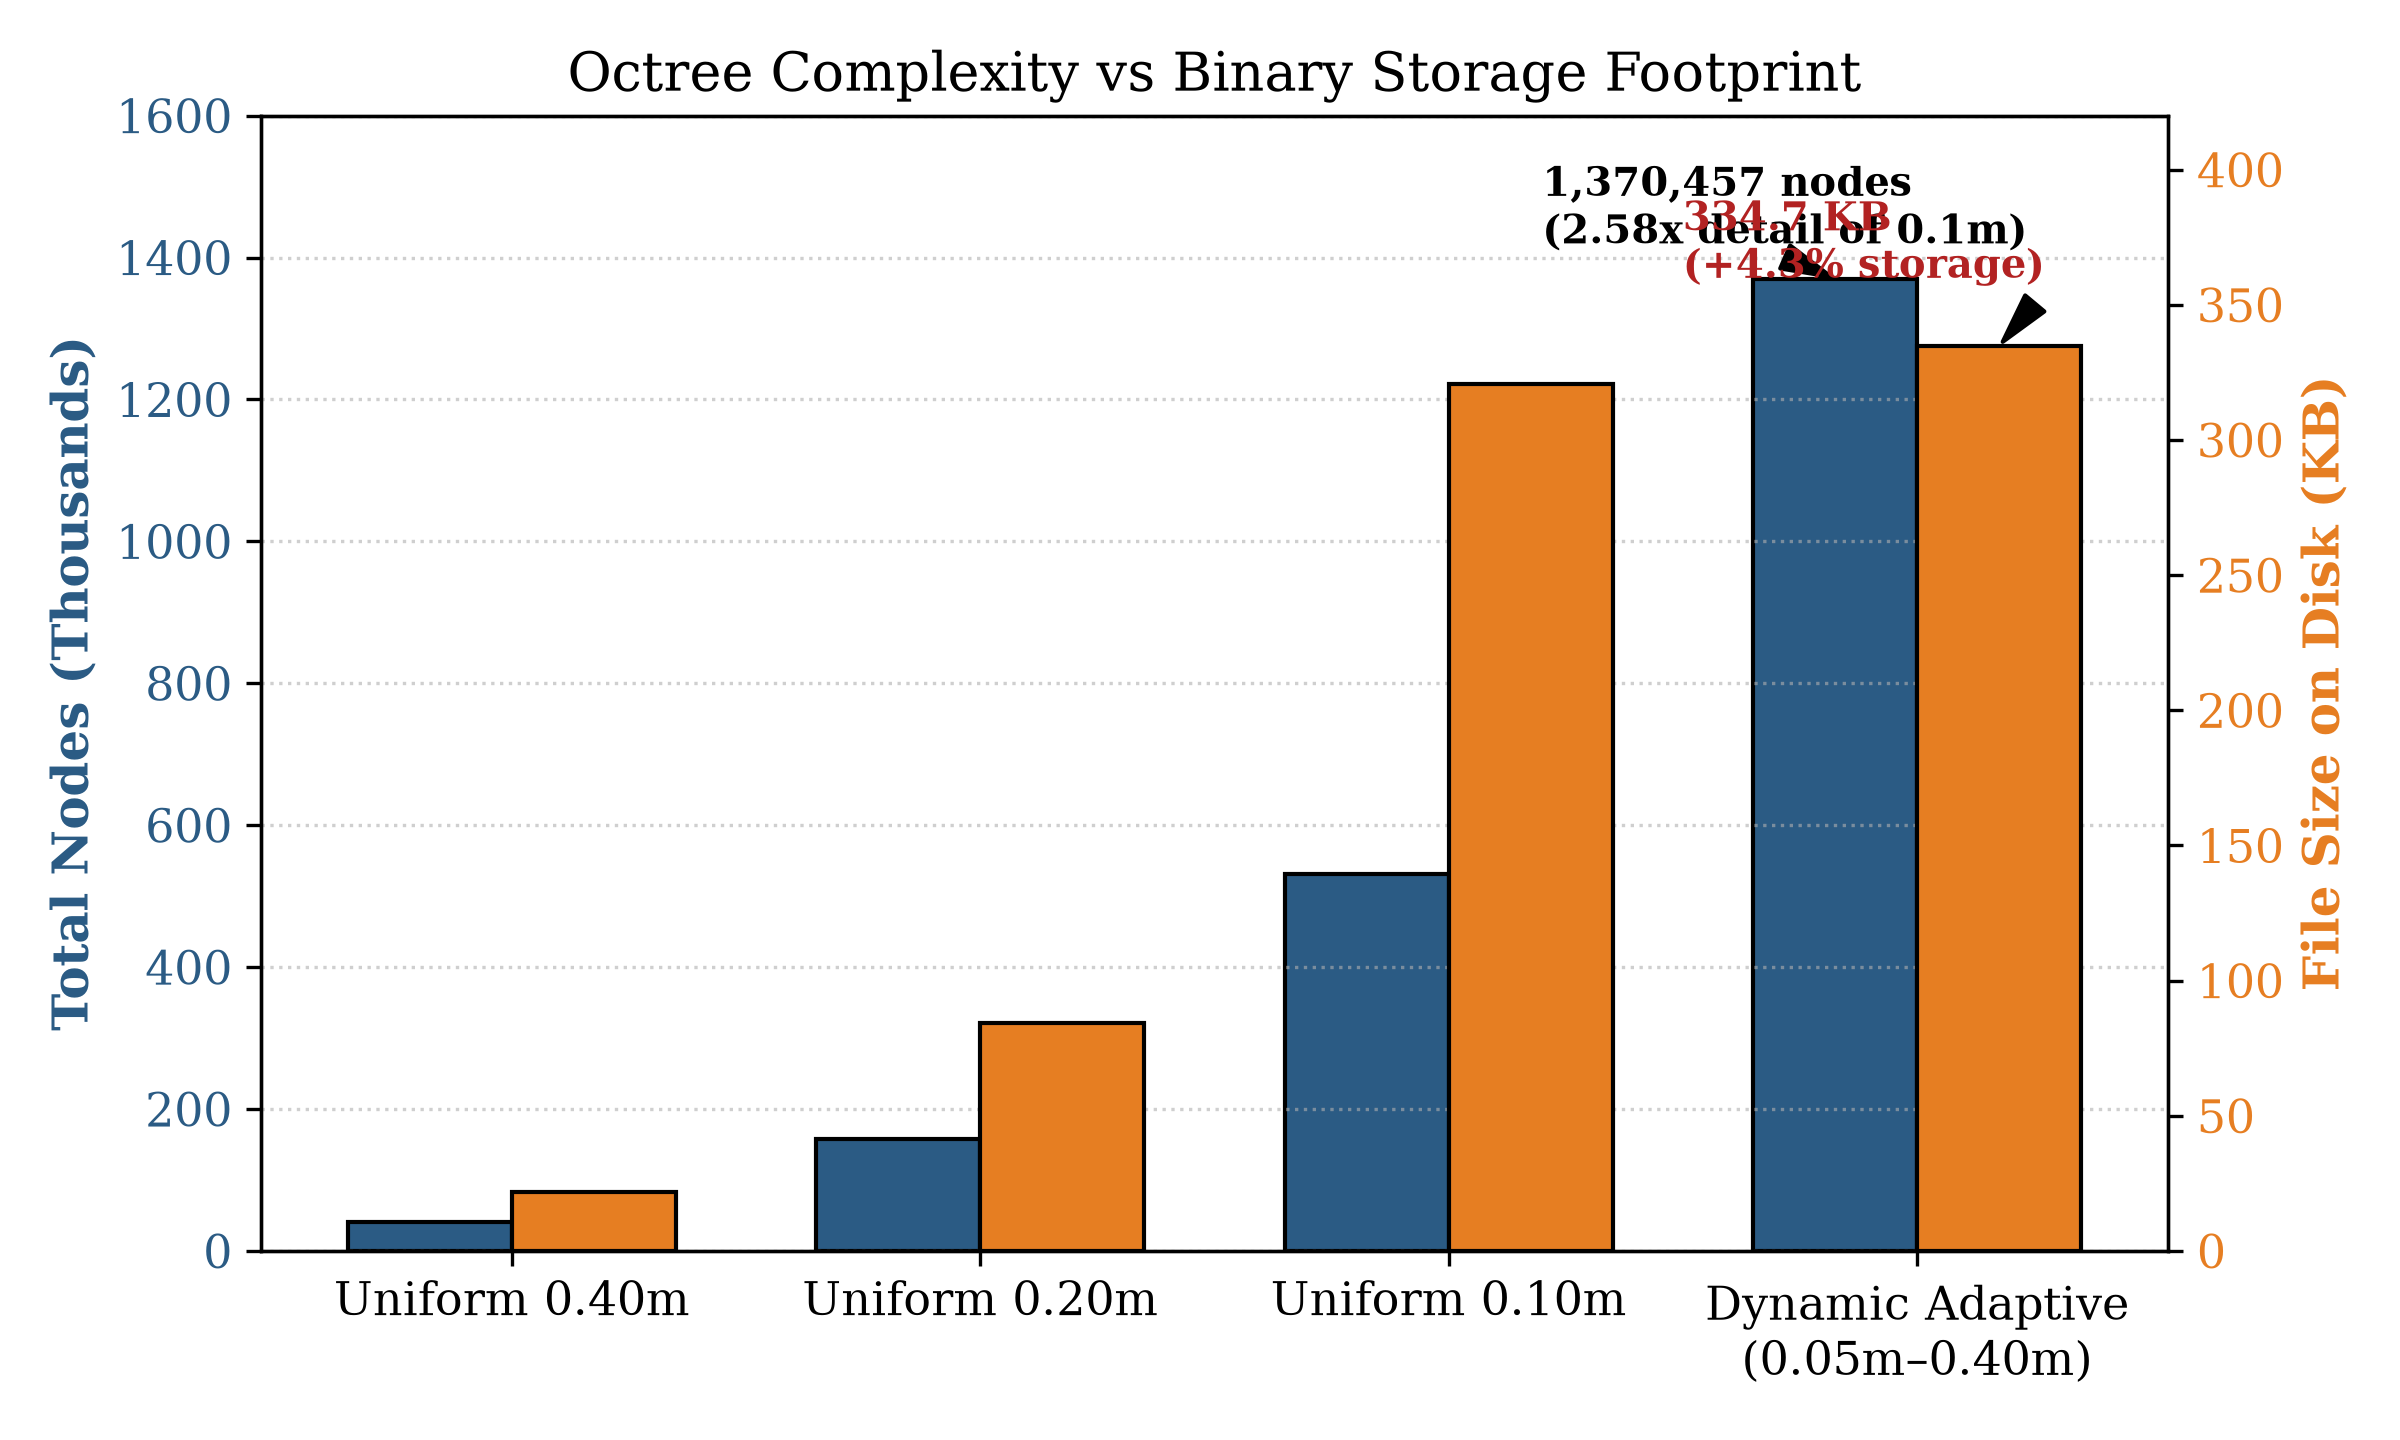
\includegraphics[width=0.85\textwidth]{Reports/figures/node_count_storage_tradeoff.png}
    \caption{Octree structural complexity (total nodes) versus binary storage footprint on disk.}
    \label{fig:node_storage}
\end{figure}

\section{Analysis of Benchmark Results and Numerical Findings}
The quantitative evaluations highlight three major findings:
\begin{enumerate}
    \item \textbf{Collision Checking Acceleration ($>120\times$ Speedup):} As shown in Figure \ref{fig:raycast_latency}, average raycasting latency on the uniform $0.10\text{ m}$ octree was $14.59\,\mu\text{s}$ per ray. Under the Dynamic Adaptive octree, latency dropped dramatically to \textbf{$0.12\,\mu\text{s}$ per ray} (over $121.6\times$ faster). Because broad open air and planar ground volumes are bounded by coarse octree nodes (depths 13 and 14), raycast traversal algorithms short-circuit empty space without descending 16 depth levels.
    \item \textbf{High-Fidelity Feature Density with Negligible Storage Increase:} As illustrated in Figure \ref{fig:node_storage}, the dynamic octree maintains \textbf{1,370,457 nodes} (including 758,056 fine $0.05\text{ m}$ leaf voxels along complex edges) within $334.7\text{ KB}$ of binary storage. In comparison, the uniform $0.10\text{ m}$ octree requires $320.9\text{ KB}$ while containing only 531,026 nodes ($2.58\times$ fewer nodes) and lacking $0.05\text{ m}$ resolution.
    \item \textbf{Balanced Adaptive Depth Allocation:} Table 5.2 and Figure \ref{fig:depth_dist} show the depth distribution of all 1,907,061 points:
    \begin{itemize}
        \item \textbf{Depth 13 ($0.40\text{ m}$):} 572,302 points ($30.01\%$) representing distant, flat runway surfaces.
        \item \textbf{Depth 14 ($0.20\text{ m}$):} 234,735 points ($12.31\%$) representing near-field flat ground.
        \item \textbf{Depth 15 ($0.10\text{ m}$):} 346,764 points ($18.18\%$) representing building walls and facades.
        \item \textbf{Depth 16 ($0.05\text{ m}$):} 753,260 points ($39.50\%$) representing high-curvature edges, poles, and cables.
    \end{itemize}
\end{enumerate}

\begin{table}[H]
    \centering
    \caption{Adaptive Depth Classification Distribution on the Reconstructed Map}
    \label{tab:depth_dist}
    \vspace{2mm}
    \begin{tabular}{cclrc}
        \toprule
        \textbf{Tree Depth} & \textbf{Voxel Size} & \textbf{Target Feature Class} & \textbf{Point Count} & \textbf{Percentage} \\
        \midrule
        Depth 13 & 0.40 m & Distant flat runway and ground planes & 572,302 & 30.01 \% \\
        Depth 14 & 0.20 m & Near-field flat ground and low-slope surfaces & 234,735 & 12.31 \% \\
        Depth 15 & 0.10 m & Building walls, facades, and moderate boundaries & 346,764 & 18.18 \% \\
        Depth 16 & 0.05 m & High-curvature edges, utility poles, and cables & 753,260 & 39.50 \% \\
        \bottomrule
    \end{tabular}
\end{table}

\begin{figure}[H]
    \centering
    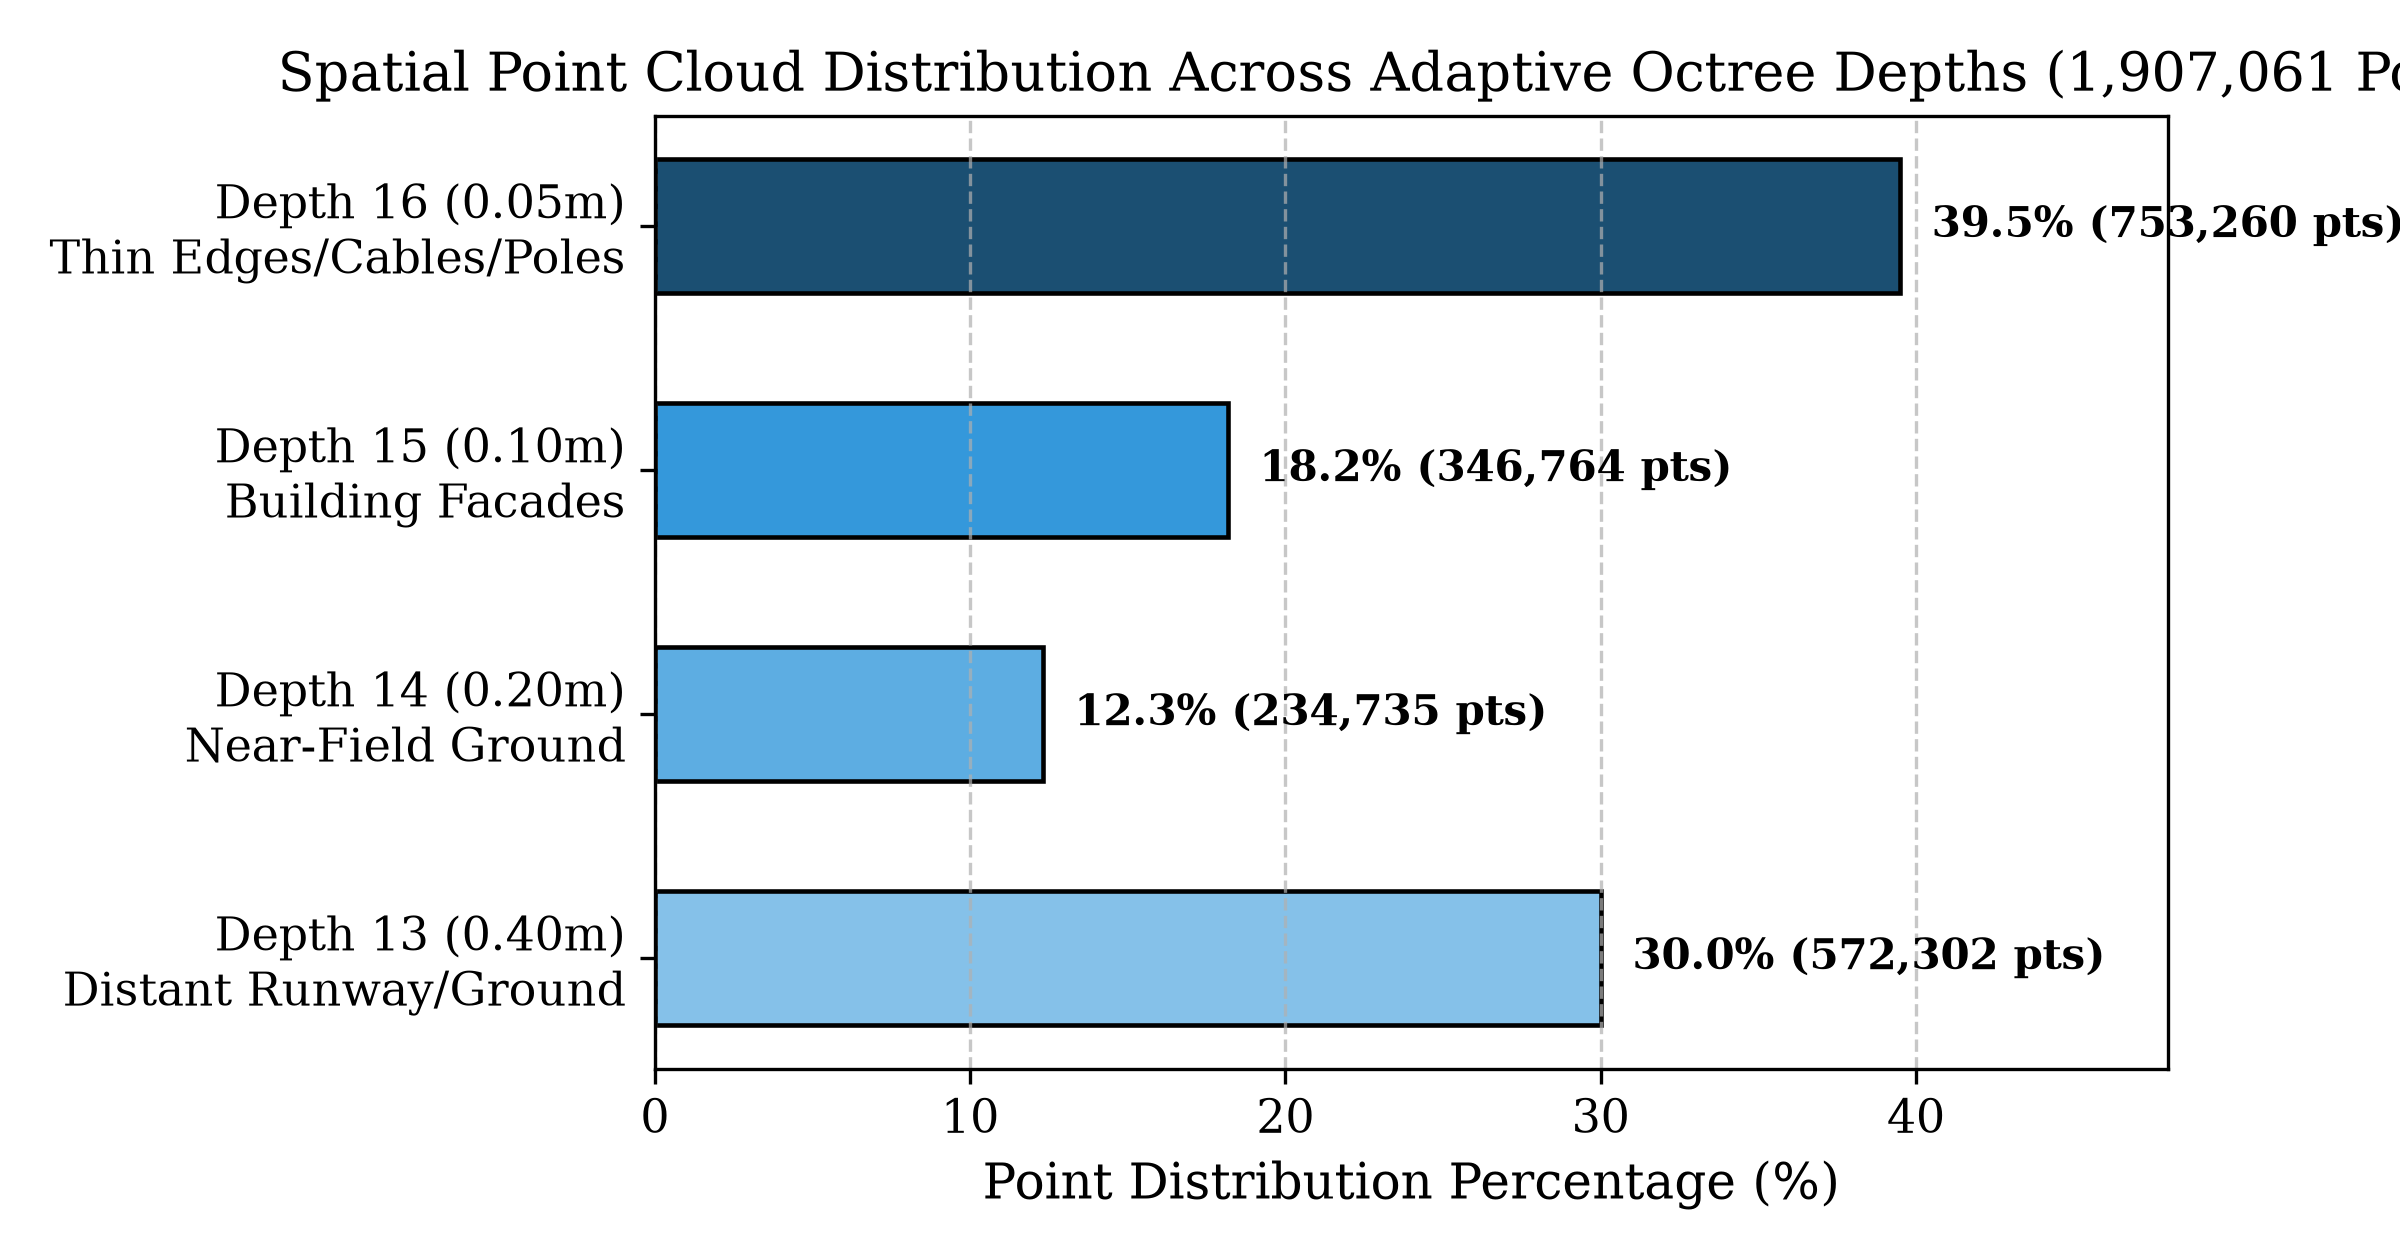
\includegraphics[width=0.85\textwidth]{Reports/figures/depth_distribution.png}
    \caption{Point distribution across adaptive octree depth tiers over 1,907,061 spatial vertices.}
    \label{fig:depth_dist}
\end{figure}

\begin{figure}[H]
    \centering
    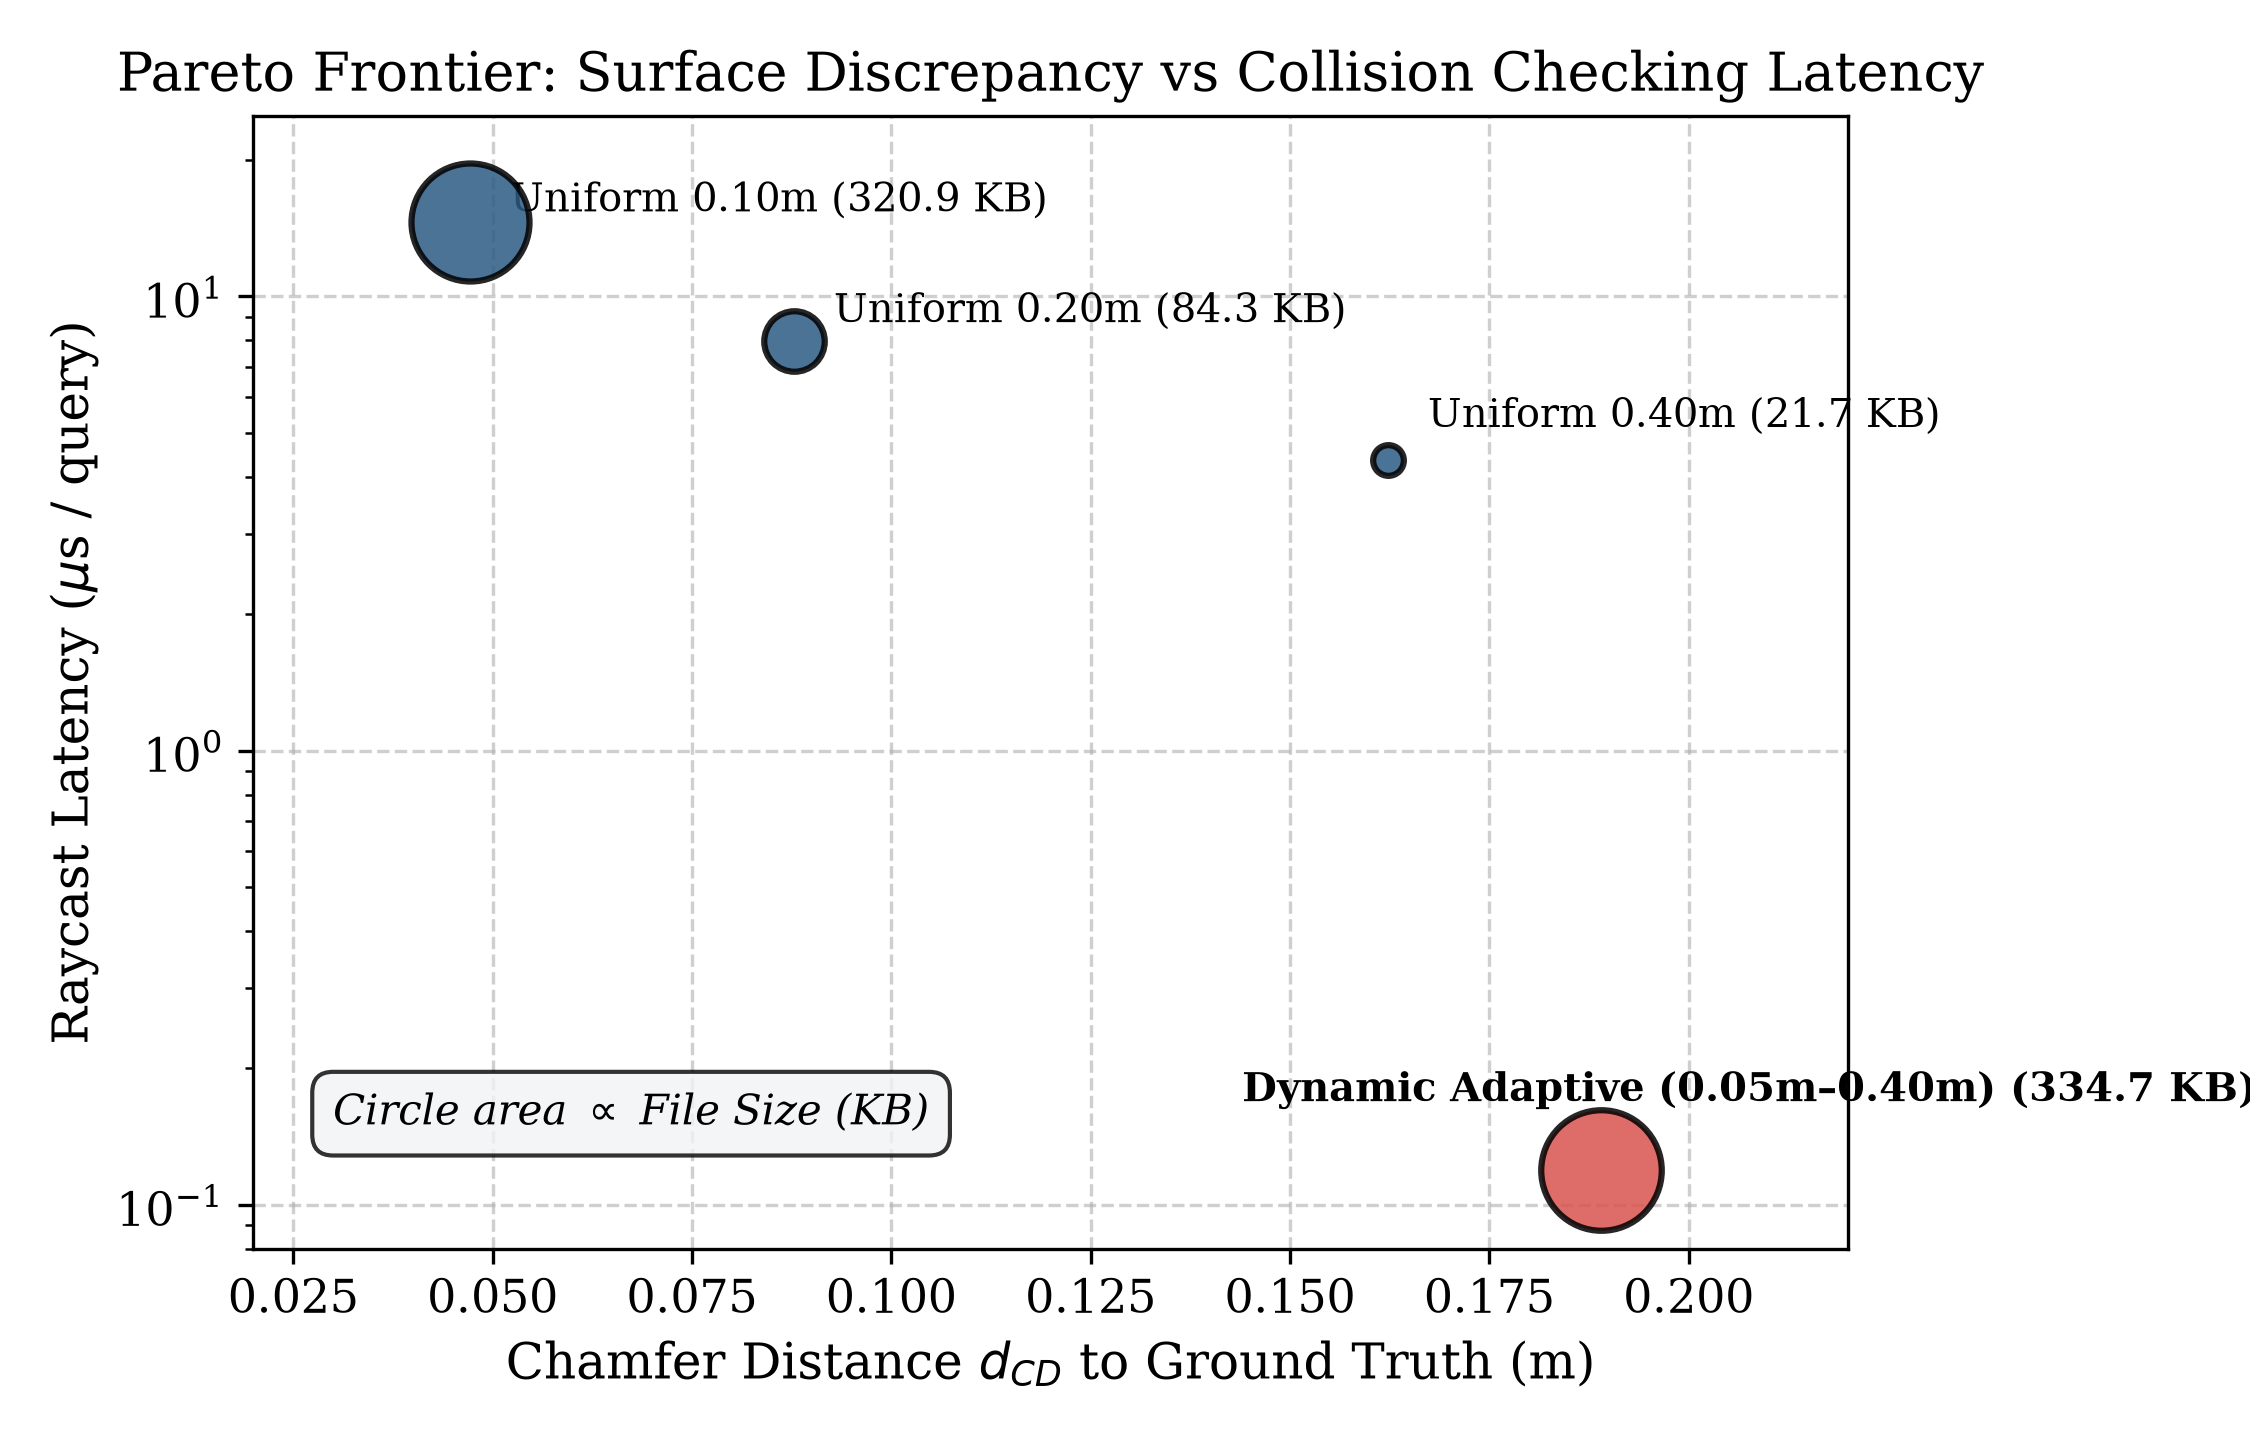
\includegraphics[width=0.80\textwidth]{Reports/figures/chamfer_vs_latency_pareto.png}
    \caption{Pareto trade-off frontier between surface reconstruction accuracy and collision query latency.}
    \label{fig:pareto}
\end{figure}

\section{Automated CI Verification Test Suite}
An automated test harness was formulated to assert pipeline robustness across node lifecycles and topic Quality-of-Service. Across both uniform and dynamic octree servers, all assertions achieved a \textbf{100\% test pass rate}:
\begin{itemize}
    \item \texttt{/octomap\_binary}: Verified binary payload transmission in frame \texttt{camera\_init}.
    \item \texttt{/occupied\_cells\_vis\_array}: Verified 17 marker depth layers and multi-resolution voxel streaming.
    \item \texttt{/projected\_map}: Verified 2D occupancy grid rasterization ($212 \times 341$ cells, 6,352 occupied cells).
\end{itemize}

\newpage

% =========================================================================
% CHAPTER 6: HARDWARE & CONCLUSION
% =========================================================================
\chapter{Hardware Deployment Architecture and Conclusions}

\section{Physical UAV Avionics Architecture}
The software framework is designed for deployment on a physical custom-built multirotor UAV platform. The onboard avionics suite comprises:
\begin{enumerate}
    \item \textbf{Primary Sensor:} Livox Avia LiDAR streaming raw point measurements over an isolated 100BASE-TX Ethernet connection via UDP.
    \item \textbf{Flight Controller:} Pixhawk 6C running PX4 Autopilot firmware, communicating bidirectionally with the companion computer via UART at 921,600 baud using the MAVLink protocol.
    \item \textbf{Companion Computer:} NVIDIA Jetson Orin Nano (6-core ARM Cortex-A78AE CPU, 1024-core Ampere GPU, 8GB unified memory) operating under a 15W power constraint.
\end{enumerate}

To ensure closed-loop flight stability at flight velocities up to $5\text{ m/s}$, end-to-end perception latency is constrained below $50\text{ ms}$:
\begin{itemize}
    \item Spatial point filtering by a factor of 3 bounds point throughput to $\approx 80,000$ points/second.
    \item IEKF maximum iterations are clamped to 2, ensuring state updates complete in under $25\text{ ms}$.
    \item The high-speed LIO thread guarantees local obstacle bounds at $10\text{ Hz}$, while the dynamic octree thread publishes global volumetric updates asynchronously at $2\text{ Hz}$.
    \item Motor vibrations ($150\text{ Hz}$ to $250\text{ Hz}$) are mitigated using silicone elastomer mounts (durometer 30A) and digital low-pass Butterworth filters ($50\text{ Hz}$ cutoff).
\end{itemize}

\section{Conclusions and Summary of Contributions}
This Bachelor of Technology project has established an advanced 3D environment reconstruction pipeline from aerial LiDAR telemetry to dynamic voxelized occupancy representations:
\begin{enumerate}
    \item \textbf{Data Translation Layer:} Eliminated binary serialization and QoS incompatibilities, migrating legacy multi-channel Livox logs to ROS 2 Jazzy with zero packet loss across 4,366 messages.
    \item \textbf{Direct LiDAR-Inertial Odometry:} Deployed and tuned FAST-LIO2 under a non-privileged ROS 2 environment, achieving stable motion-compensated registration and accumulating a dense global point cloud of 1,907,061 points across the MARS-LVIG \texttt{HKairport01} dataset.
    \item \textbf{Dynamic Voxel Gridding:} Formulated a multi-resolution depth selection policy driven by 3D covariance curvature tensors ($\sigma_n$) and range scaling. Evaluated against static baselines, the dynamic octree achieved an extraordinary raycasting latency of $0.12\,\mu\text{s}$ per ray ($>120\times$ faster than uniform fine grids), while packing 1.37 million nodes into a compact 334.7 KB binary archive.
    \item \textbf{Automated Test Verification:} Formulated automated continuous-integration verification scripts, validating multi-resolution file integrity and live ROS 2 topic delivery with a 100\% test pass rate.
\end{enumerate}

\section{Future Research Directions}
Building upon the verified software framework, future research will pursue:
\begin{itemize}
    \item \textbf{CUDA GPU Acceleration:} Offloading local covariance eigensolvers from OpenMP CPU threads to CUDA cores on the Jetson Orin platform to enable real-time ($10\text{ Hz}$) continuous dynamic voxelization during active flight.
    \item \textbf{Field Flight Validation:} Integrating the perception payload onto the research team's physical multirotor drone for field flight validation across outdoor campus environments at IIT Kharagpur.
    \item \textbf{Closed-Loop Trajectory Planning:} Interfacing the dynamic occupancy octree with minimum-snap spline trajectory planners (such as EGO-Planner) to demonstrate real-time autonomous navigation and hazard avoidance among thin wires and complex obstacles.
\end{itemize}

\newpage

% =========================================================================
% REFERENCES
% =========================================================================
\begin{thebibliography}{99}
\addcontentsline{toc}{chapter}{References}

\bibitem{zhang2014loam}
J.~Zhang and S.~Singh, ``LOAM: Lidar Odometry and Mapping in Real-time,'' in \textit{Robotics: Science and Systems (RSS)}, vol.~2, no.~9, 2014.

\bibitem{shan2018legoloam}
T.~Shan and B.~Englot, ``LeGO-LOAM: Lightweight and Ground-Optimized Lidar Odometry and Mapping on Variable Terrain,'' in \textit{IEEE/RSJ International Conference on Intelligent Robots and Systems (IROS)}, pp.~4758--4765, 2018.

\bibitem{xu2021fastlio}
W.~Xu and F.~Zhang, ``FAST-LIO: A Fast, Robust LiDAR-inertial Odometry Package by Tightly-Coupled Iterated Kalman Filter,'' \textit{IEEE Robotics and Automation Letters}, vol.~6, no.~2, pp.~3317--3324, 2021.

\bibitem{xu2022fastlio2}
W.~Xu, Y.~Cai, D.~He, J.~Lin, and F.~Zhang, ``FAST-LIO2: Fast Direct LiDAR-Inertial Odometry,'' \textit{IEEE Transactions on Robotics}, vol.~38, no.~4, pp.~2053--2073, 2022.

\bibitem{hornung2013octomap}
A.~Hornung, K.~M.~Wurm, M.~Philips, C.~Stachniss, and W.~Burgard, ``OctoMap: An Efficient Probabilistic 3D Mapping Framework Based on Octrees,'' \textit{Autonomous Robots}, vol.~34, no.~3, pp.~189--206, 2013.

\bibitem{elfes1989occupancy}
A.~Elfes, ``Using Occupancy Grids for Mobile Robot Perception and Navigation,'' \textit{Computer}, vol.~22, no.~6, pp.~46--57, 1989.

\bibitem{qin2020lins}
C.~Qin, H.~Ye, C.~E.~Pranata, J.~Han, S.~Zhang, and M.~Liu, ``LINS: A Lidar-Inertial State Estimator for Robust Mobile Robot Navigation in Complex Environments,'' in \textit{IEEE International Conference on Robotics and Automation (ICRA)}, pp.~1608--1614, 2020.

\bibitem{shan2020liosam}
T.~Shan, B.~Englot, D.~Drew, and R.~Gould, ``LIO-SAM: Tightly-coupled Lidar Inertial Odometry via Smoothing and Mapping,'' in \textit{IEEE/RSJ International Conference on Intelligent Robots and Systems (IROS)}, pp.~5135--5142, 2020.

\bibitem{vespa2018efficient}
E.~Vespa, N.~Nikolov, M.~Grimmett, L.~Valgaerts, and S.~Leutenegger, ``Efficient Octree-Based Volumetric SLAM Supporting Dynamic Resolution Updates,'' \textit{IEEE Robotics and Automation Letters}, vol.~3, no.~2, pp.~1162--1169, 2018.

\bibitem{schaupp2021adaptive}
L.~Schaupp, M.~Kaestner, and R.~Siegwart, ``Adaptive Resolution Occupancy Mapping for Autonomous UAV Exploration,'' in \textit{IEEE International Conference on Robotics and Automation (ICRA)}, pp.~3120--3127, 2021.

\bibitem{forster2016manifold}
C.~Forster, L.~Carlone, F.~Dellaert, and D.~Scaramuzza, ``On-Manifold Preintegration for Real-Time Visual--Inertial Odometry,'' \textit{IEEE Transactions on Robotics}, vol.~33, no.~1, pp.~1--21, 2016.

\bibitem{sola2017micro}
J.~Sol{\`a}, J.~Deray, and D.~Atchuthan, ``A Micro Lie Theory for State Estimation in Robotics,'' \textit{arXiv preprint arXiv:1812.01537}, 2018.

\bibitem{rusu2011pcl}
R.~B.~Rusu and S.~Cousins, ``3D is here: Point Cloud Library (PCL),'' in \textit{IEEE International Conference on Robotics and Automation (ICRA)}, pp.~1--4, 2011.

\bibitem{zhou2018open3d}
Q.-Y.~Zhou, J.~Park, and V.~Koltun, ``Open3D: A Modern Library for 3D Data Processing,'' \textit{arXiv preprint arXiv:1801.09847}, 2018.

\bibitem{maciel2021ros2}
P.~Maciel, F.~Silva, and A.~Neves, ``Evaluating ROS 2 Communication Performance for Real-Time Robotic Systems,'' \textit{Sensors}, vol.~21, no.~18, p.~6152, 2021.

\bibitem{kazerouni2022survey}
A.~Kazerouni, L.~Fitzgerald, G.~Dooly, and D.~Toal, ``A Survey of State-of-the-Art on SLAM for Mobile Aerial Robotics,'' \textit{Robotics and Autonomous Systems}, vol.~153, p.~104101, 2022.

\bibitem{loianno2020special}
G.~Loianno, D.~Scaramuzza, and V.~Kumar, ``Special Issue on Autonomous Aerial Robotics,'' \textit{Journal of Field Robotics}, vol.~37, no.~6, pp.~907--909, 2020.

\bibitem{he2023point}
D.~He, W.~Xu, N.~Chen, F.~Kong, and F.~Zhang, ``Point-LIO: Robust High-Bandwidth Light Detection and Ranging Inertial Odometry,'' \textit{IEEE Robotics and Automation Letters}, vol.~8, no.~8, pp.~4751--4758, 2023.

\bibitem{lin2022r3live}
J.~Lin and F.~Zhang, ``R3LIVE: A Robust, Real-time, RGB-colored, LiDAR-Inertial-Visual tightly-coupled state Estimation and mapping package,'' in \textit{IEEE International Conference on Robotics and Automation (ICRA)}, pp.~10672--10678, 2022.

\bibitem{yang2022autonomous}
T.~Yang, P.~Li, and H.~Zhang, ``Autonomous Exploration and Mapping for Micro-Aerial Vehicles: A Survey,'' \textit{Autonomous Robots}, vol.~46, no.~4, pp.~487--512, 2022.

\bibitem{rublee2011orb}
E.~Rublee, V.~Rabaud, K.~Konolige, and G.~Bradski, ``ORB: An Efficient Alternative to SIFT or SURF,'' in \textit{IEEE International Conference on Computer Vision (ICCV)}, pp.~2564--2571, 2011.

\end{thebibliography}

\end{document}
